\documentclass{standalone}

\usepackage{tikz}
\usepackage{circuitikz}

\tikzset{block/.style = {draw, fill=white, very thick, rectangle, minimum height=1cm, minimum width=2cm},
         lblock/.style={draw,fill=white,very thick, rectangle, minimum height=3cm, minimum width=1cm},
         sum/.style= {draw, fill=white, very thick, circle, node distance=0.5cm}}

         
\begin{document}
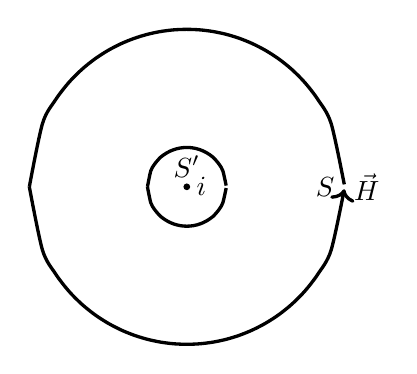
\begin{tikzpicture}[scale=2]
    \draw[-,very thick]plot[smooth, domain=-1:1](\x,{(1-(\x)^2)^0.5});
    \draw[->,very thick]plot[smooth, domain=-1:1](\x,{-(1-(\x)^2)^0.5});
    \node[right]at(1,0){$\vec{H}$};
    \node[left]at(1,0){$S$};

    \draw[-, very thick]plot[smooth, domain=-0.25:0.25](\x,{(0.0625-(\x)^2)^0.5});
    \draw[-, very thick]plot[smooth, domain=-0.25:0.25](\x,{-(0.0625-(\x)^2)^0.5});
    \node[right]at(0,0){$i$}node[above]{$S'$};
    \filldraw[black](0,0)circle(0.5pt);
\end{tikzpicture}
\end{document}